% Options for packages loaded elsewhere
\PassOptionsToPackage{unicode}{hyperref}
\PassOptionsToPackage{hyphens}{url}
%
\documentclass[
]{article}
\usepackage{amsmath,amssymb}
\usepackage{iftex}
\ifPDFTeX
  \usepackage[T1]{fontenc}
  \usepackage[utf8]{inputenc}
  \usepackage{textcomp} % provide euro and other symbols
\else % if luatex or xetex
  \usepackage{unicode-math} % this also loads fontspec
  \defaultfontfeatures{Scale=MatchLowercase}
  \defaultfontfeatures[\rmfamily]{Ligatures=TeX,Scale=1}
\fi
\usepackage{lmodern}
\ifPDFTeX\else
  % xetex/luatex font selection
\fi
% Use upquote if available, for straight quotes in verbatim environments
\IfFileExists{upquote.sty}{\usepackage{upquote}}{}
\IfFileExists{microtype.sty}{% use microtype if available
  \usepackage[]{microtype}
  \UseMicrotypeSet[protrusion]{basicmath} % disable protrusion for tt fonts
}{}
\makeatletter
\@ifundefined{KOMAClassName}{% if non-KOMA class
  \IfFileExists{parskip.sty}{%
    \usepackage{parskip}
  }{% else
    \setlength{\parindent}{0pt}
    \setlength{\parskip}{6pt plus 2pt minus 1pt}}
}{% if KOMA class
  \KOMAoptions{parskip=half}}
\makeatother
\usepackage{xcolor}
\usepackage{color}
\usepackage{fancyvrb}
\newcommand{\VerbBar}{|}
\newcommand{\VERB}{\Verb[commandchars=\\\{\}]}
\DefineVerbatimEnvironment{Highlighting}{Verbatim}{commandchars=\\\{\}}
% Add ',fontsize=\small' for more characters per line
\newenvironment{Shaded}{}{}
\newcommand{\AlertTok}[1]{\textcolor[rgb]{1.00,0.00,0.00}{\textbf{#1}}}
\newcommand{\AnnotationTok}[1]{\textcolor[rgb]{0.38,0.63,0.69}{\textbf{\textit{#1}}}}
\newcommand{\AttributeTok}[1]{\textcolor[rgb]{0.49,0.56,0.16}{#1}}
\newcommand{\BaseNTok}[1]{\textcolor[rgb]{0.25,0.63,0.44}{#1}}
\newcommand{\BuiltInTok}[1]{\textcolor[rgb]{0.00,0.50,0.00}{#1}}
\newcommand{\CharTok}[1]{\textcolor[rgb]{0.25,0.44,0.63}{#1}}
\newcommand{\CommentTok}[1]{\textcolor[rgb]{0.38,0.63,0.69}{\textit{#1}}}
\newcommand{\CommentVarTok}[1]{\textcolor[rgb]{0.38,0.63,0.69}{\textbf{\textit{#1}}}}
\newcommand{\ConstantTok}[1]{\textcolor[rgb]{0.53,0.00,0.00}{#1}}
\newcommand{\ControlFlowTok}[1]{\textcolor[rgb]{0.00,0.44,0.13}{\textbf{#1}}}
\newcommand{\DataTypeTok}[1]{\textcolor[rgb]{0.56,0.13,0.00}{#1}}
\newcommand{\DecValTok}[1]{\textcolor[rgb]{0.25,0.63,0.44}{#1}}
\newcommand{\DocumentationTok}[1]{\textcolor[rgb]{0.73,0.13,0.13}{\textit{#1}}}
\newcommand{\ErrorTok}[1]{\textcolor[rgb]{1.00,0.00,0.00}{\textbf{#1}}}
\newcommand{\ExtensionTok}[1]{#1}
\newcommand{\FloatTok}[1]{\textcolor[rgb]{0.25,0.63,0.44}{#1}}
\newcommand{\FunctionTok}[1]{\textcolor[rgb]{0.02,0.16,0.49}{#1}}
\newcommand{\ImportTok}[1]{\textcolor[rgb]{0.00,0.50,0.00}{\textbf{#1}}}
\newcommand{\InformationTok}[1]{\textcolor[rgb]{0.38,0.63,0.69}{\textbf{\textit{#1}}}}
\newcommand{\KeywordTok}[1]{\textcolor[rgb]{0.00,0.44,0.13}{\textbf{#1}}}
\newcommand{\NormalTok}[1]{#1}
\newcommand{\OperatorTok}[1]{\textcolor[rgb]{0.40,0.40,0.40}{#1}}
\newcommand{\OtherTok}[1]{\textcolor[rgb]{0.00,0.44,0.13}{#1}}
\newcommand{\PreprocessorTok}[1]{\textcolor[rgb]{0.74,0.48,0.00}{#1}}
\newcommand{\RegionMarkerTok}[1]{#1}
\newcommand{\SpecialCharTok}[1]{\textcolor[rgb]{0.25,0.44,0.63}{#1}}
\newcommand{\SpecialStringTok}[1]{\textcolor[rgb]{0.73,0.40,0.53}{#1}}
\newcommand{\StringTok}[1]{\textcolor[rgb]{0.25,0.44,0.63}{#1}}
\newcommand{\VariableTok}[1]{\textcolor[rgb]{0.10,0.09,0.49}{#1}}
\newcommand{\VerbatimStringTok}[1]{\textcolor[rgb]{0.25,0.44,0.63}{#1}}
\newcommand{\WarningTok}[1]{\textcolor[rgb]{0.38,0.63,0.69}{\textbf{\textit{#1}}}}
\usepackage{graphicx}
\makeatletter
\def\maxwidth{\ifdim\Gin@nat@width>\linewidth\linewidth\else\Gin@nat@width\fi}
\def\maxheight{\ifdim\Gin@nat@height>\textheight\textheight\else\Gin@nat@height\fi}
\makeatother
% Scale images if necessary, so that they will not overflow the page
% margins by default, and it is still possible to overwrite the defaults
% using explicit options in \includegraphics[width, height, ...]{}
\setkeys{Gin}{width=\maxwidth,height=\maxheight,keepaspectratio}
% Set default figure placement to htbp
\makeatletter
\def\fps@figure{htbp}
\makeatother
\setlength{\emergencystretch}{3em} % prevent overfull lines
\providecommand{\tightlist}{%
  \setlength{\itemsep}{0pt}\setlength{\parskip}{0pt}}
\setcounter{secnumdepth}{-\maxdimen} % remove section numbering
\ifLuaTeX
  \usepackage{selnolig}  % disable illegal ligatures
\fi
\IfFileExists{bookmark.sty}{\usepackage{bookmark}}{\usepackage{hyperref}}
\IfFileExists{xurl.sty}{\usepackage{xurl}}{} % add URL line breaks if available
\urlstyle{same}
\hypersetup{
  hidelinks,
  pdfcreator={LaTeX via pandoc}}

\author{}
\date{}

\begin{document}

\hypertarget{image-interpolation}{%
\section{Image Interpolation}\label{image-interpolation}}

\hypertarget{1-introduction}{%
\section{1 Introduction}\label{1-introduction}}

In this lab, we delve into the topic of image interpolation.
Specifically, three kinds of image interpolation methods are mainly
introduced, i.e., nearest neighbor interpolation, bilinear
interpolation, and bicubic interpolation. These three kinds of
interpolation methods all involve pixel index mapping. During the
experiment, I found inverse mapping, which maps the pixel index in the
interpolated image to the original image, is easier and more intuitive.
So, I mainly use this mapping method. The results of interpolation are
satisfying, which yields the expected effect on the image.

Keywords: nearest neighbor interpolation; bilinear interpolation;
bicubic interpolation; index mapping

\hypertarget{2-method}{%
\section{2 Method}\label{2-method}}

\hypertarget{21-nearest-neighbor-interpolation}{%
\subsection{2.1 Nearest Neighbor
Interpolation}\label{21-nearest-neighbor-interpolation}}

Nearest neighbor interpolation is perhaps the most straightforward and
also the fastest interpolation method. The most important part of the
nearest neighbor interpolation is pixel mapping. As shown in figure
\textbackslash ref\{\}, the index of the interpolated image (in brown)
can be mapped into the index of the original image (in green).
\textbf{Note that the grid points represent pixels.}

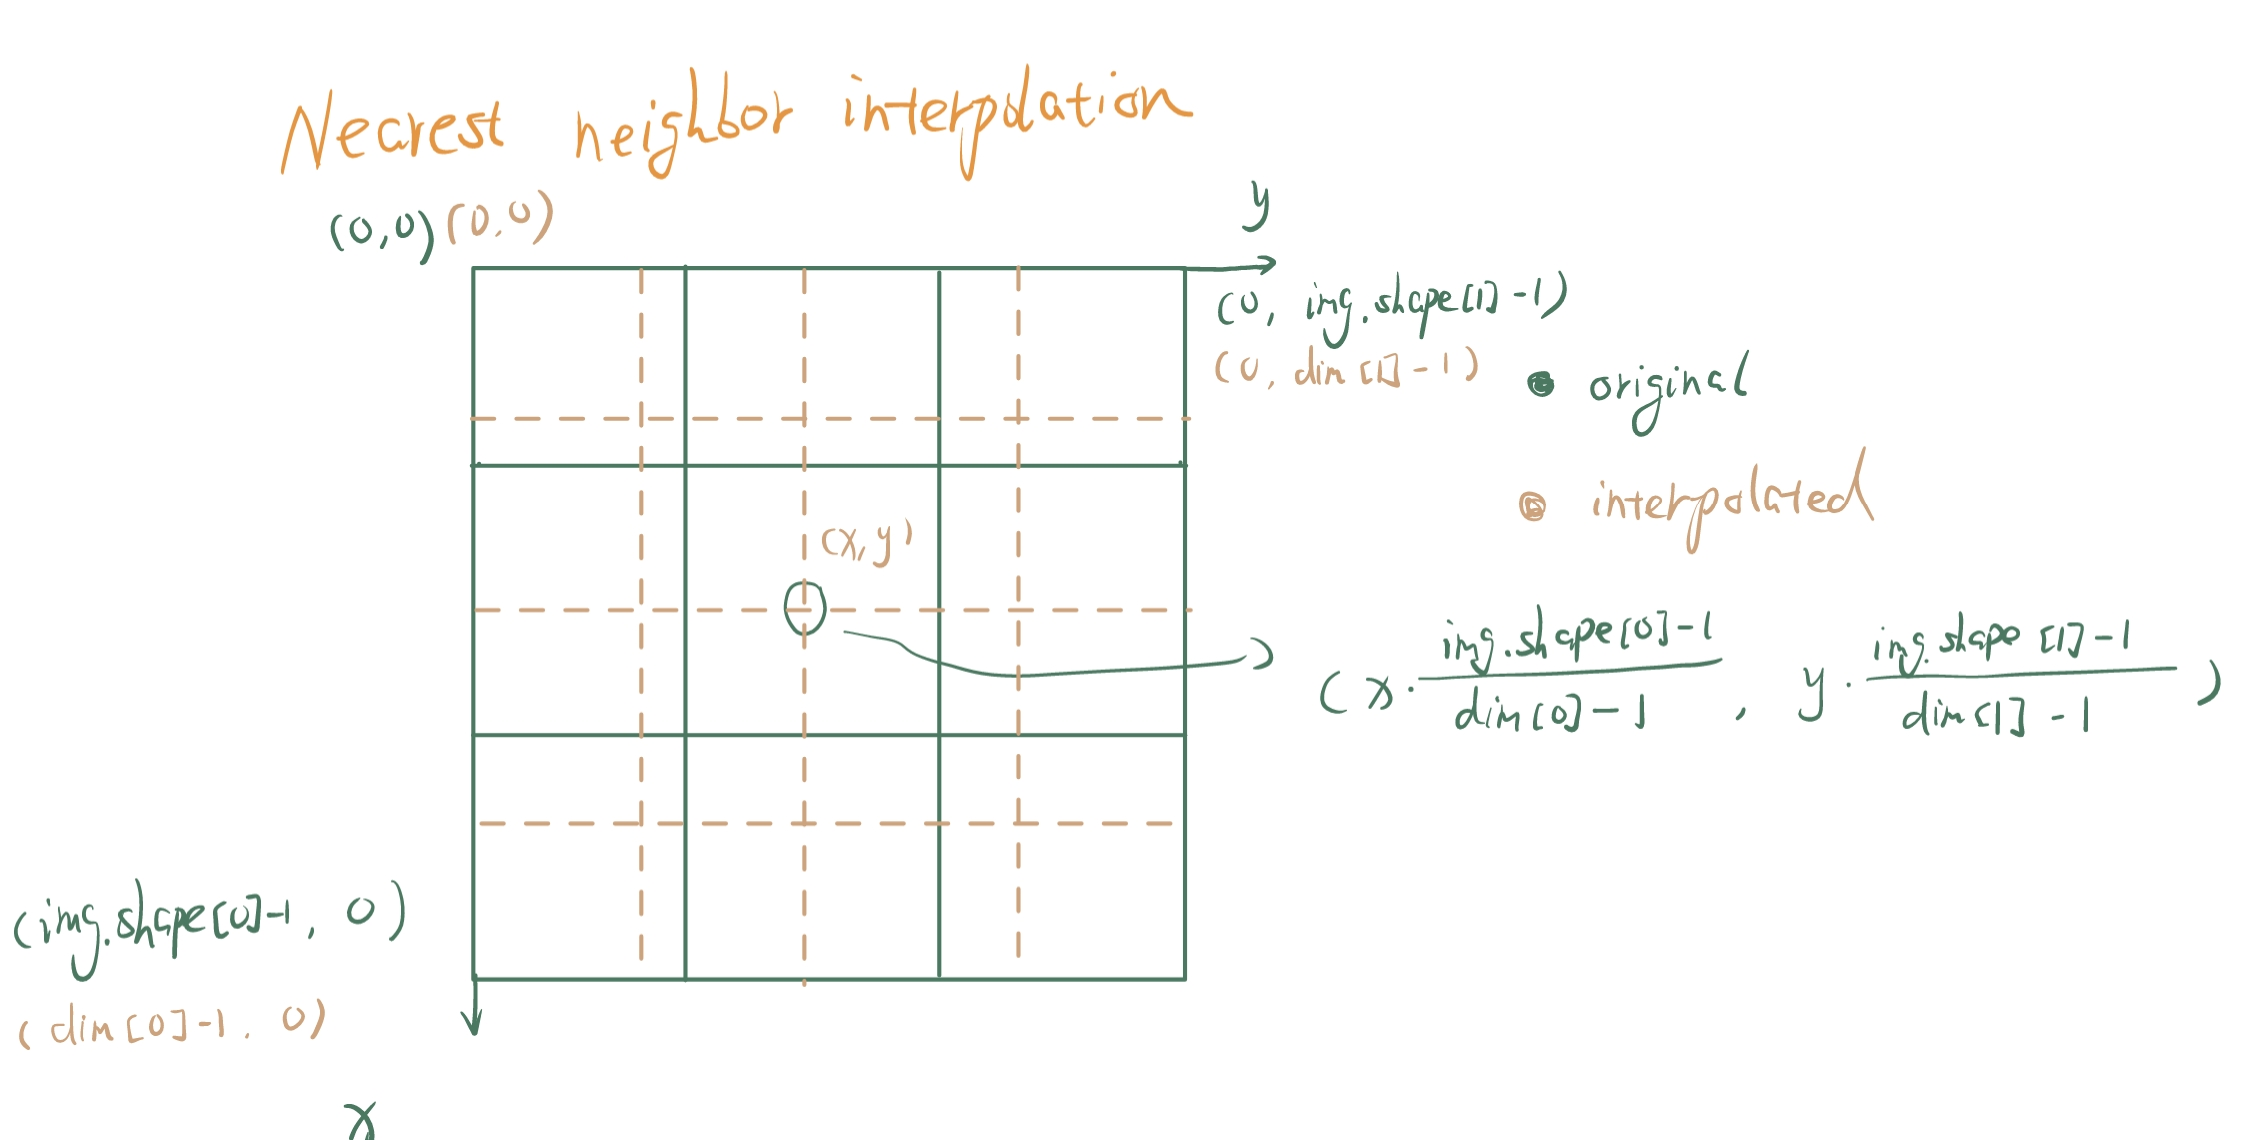
\includegraphics{D:/Tangent/SUSTech/大三下/课程资料/DIP/Lab/lab repo/Lab2/report/assets/nearest_mapping.jpg}

As for the value assignment for the interpolated image, consider the
following procedure:

\begin{enumerate}
\def\labelenumi{\arabic{enumi}.}
\item
  Get the inverse mapping index of the interpolated image in the
  original image.
\end{enumerate}

\begin{enumerate}
\def\labelenumi{\arabic{enumi}.}
\item
  Round off the x and y indexes or coordinates and get the integer
  indexes.
\end{enumerate}

\begin{enumerate}
\def\labelenumi{\arabic{enumi}.}
\item
  Assign the pixel of the interpolated image with the value where the
  pixel of the same integer indexes in the original image.
\end{enumerate}

\hypertarget{22-bilinear-interpolation}{%
\subsection{2.2 Bilinear
Interpolation}\label{22-bilinear-interpolation}}

Bilinear interpolation is a better choice of image interpolation method
if we want the interpolated image to be smooth rather than edgy. The
naive method for bilinear interpolation is that we can first interpolate
along one of the axes and then interpolate along the other.

The basic method is shown in figure \textbackslash ref\{\}.

\begin{enumerate}
\def\labelenumi{\arabic{enumi}.}
\item
  Interpolate along the y-axis to obtain the intermediate value of the
  grid points marked \texttt{x} in purple.
\item
  Then interpolate along the x-axis to obtain the exact value of the
  grid points of the interpolated image.
\end{enumerate}

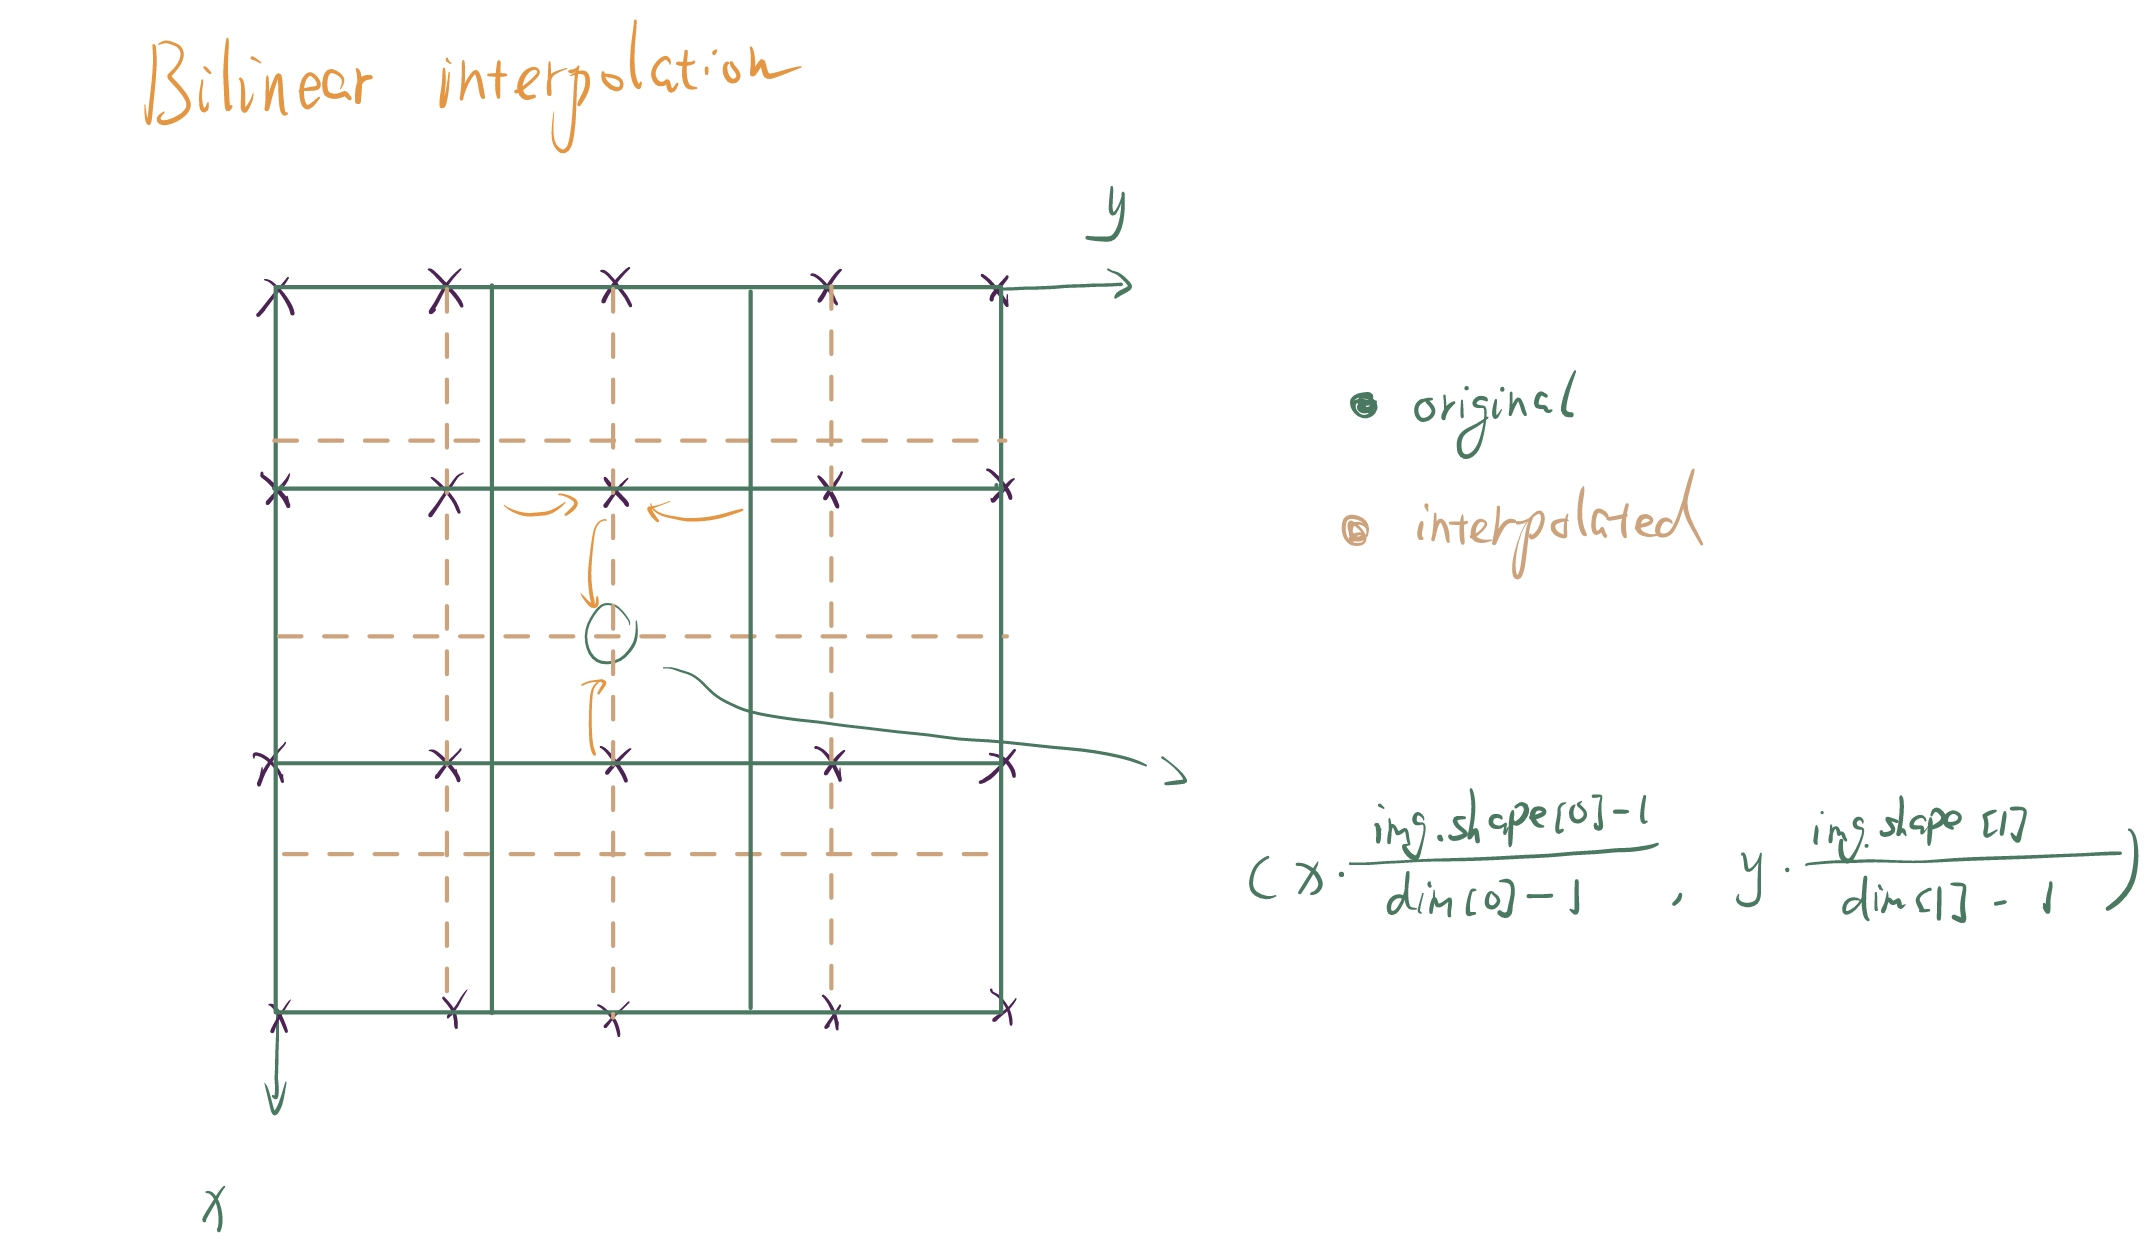
\includegraphics{D:/Tangent/SUSTech/大三下/课程资料/DIP/Lab/lab repo/Lab2/report/assets/bilinear_mapping_slow.jpg}

\hypertarget{extension-alternative-way-for-bilinear-interpolation}{%
\subsubsection{Extension: Alternative Way for Bilinear
Interpolation}\label{extension-alternative-way-for-bilinear-interpolation}}

Suppose we delve deeper into the pixel assignment of the interpolated
image. In that case, we can find out that the pixel's value of the
interpolated image only associates with the four neighbors of the
original image. So, we may ask, since it is bilinear, is there a way to
assign an interpolated pixel with only the weighted values of those four
neighbors? The answer is yes.

As shown in Figure \textbackslash ref\{\}, we can use the formula in
this figure to obtain the exact value of the interpolated pixel directly
from the four neighbors. Parameters \texttt{m} and \texttt{n} can be
easily derived from the mapped indexes of interpolated pixels.

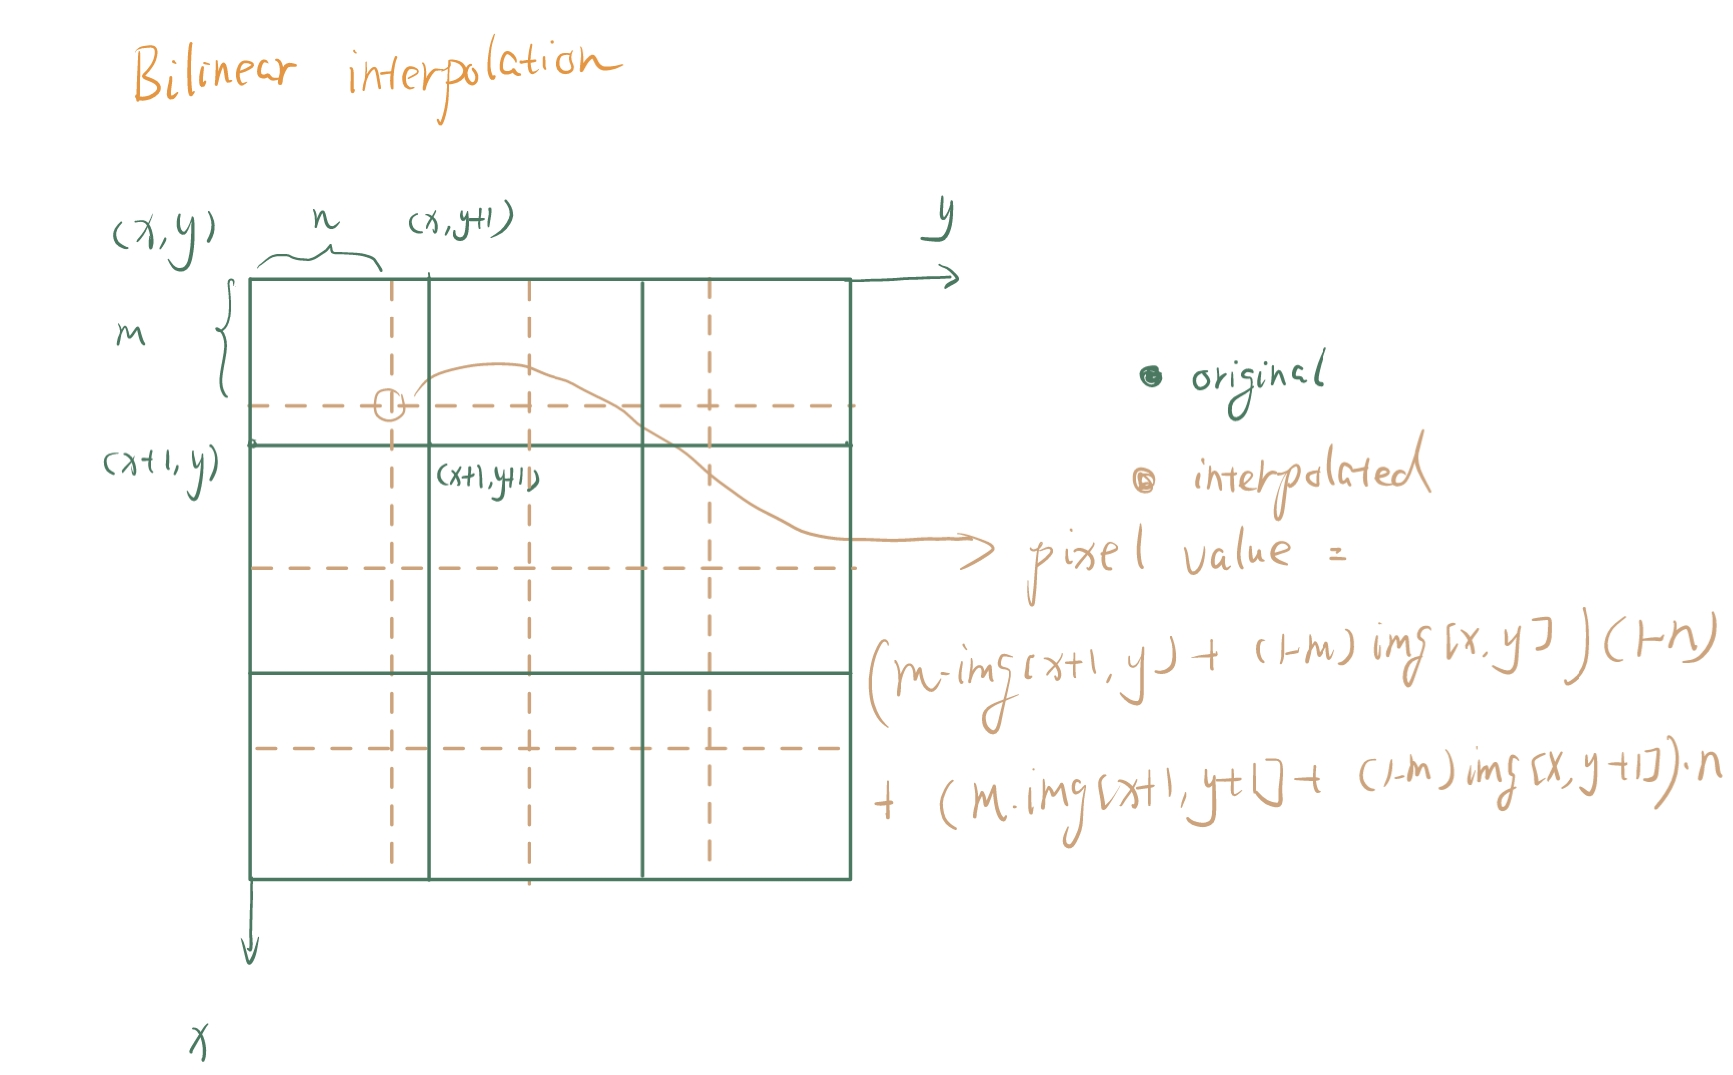
\includegraphics{D:/Tangent/SUSTech/大三下/课程资料/DIP/Lab/lab repo/Lab2/report/assets/bilinear_mapping_fast.jpg}

\hypertarget{23-bicubic-interpolation}{%
\subsection{2.3 Bicubic Interpolation}\label{23-bicubic-interpolation}}

Bicubic interpolation is the most difficult of the three interpolation
methods. The hardest part is that we need at most \(4\times4=16\) pixels
from the original image to obtain only one pixel of the interpolated
image. We also need to consider that there are not enough pixels from
the original image at the edge of the interpolated image for us to do
cubic regression. My solution is as follows, though it may seem
inefficient.

As shown in Figure \textbackslash ref\{\}, to obtain the pixel value of
the center pixel marked \texttt{o}, we need first to use cubic
regression to interpolate the intermediate pixel values marked
\texttt{x} along the y-axis, then use these intermediate pixel values to
interpolate along the x-axis.

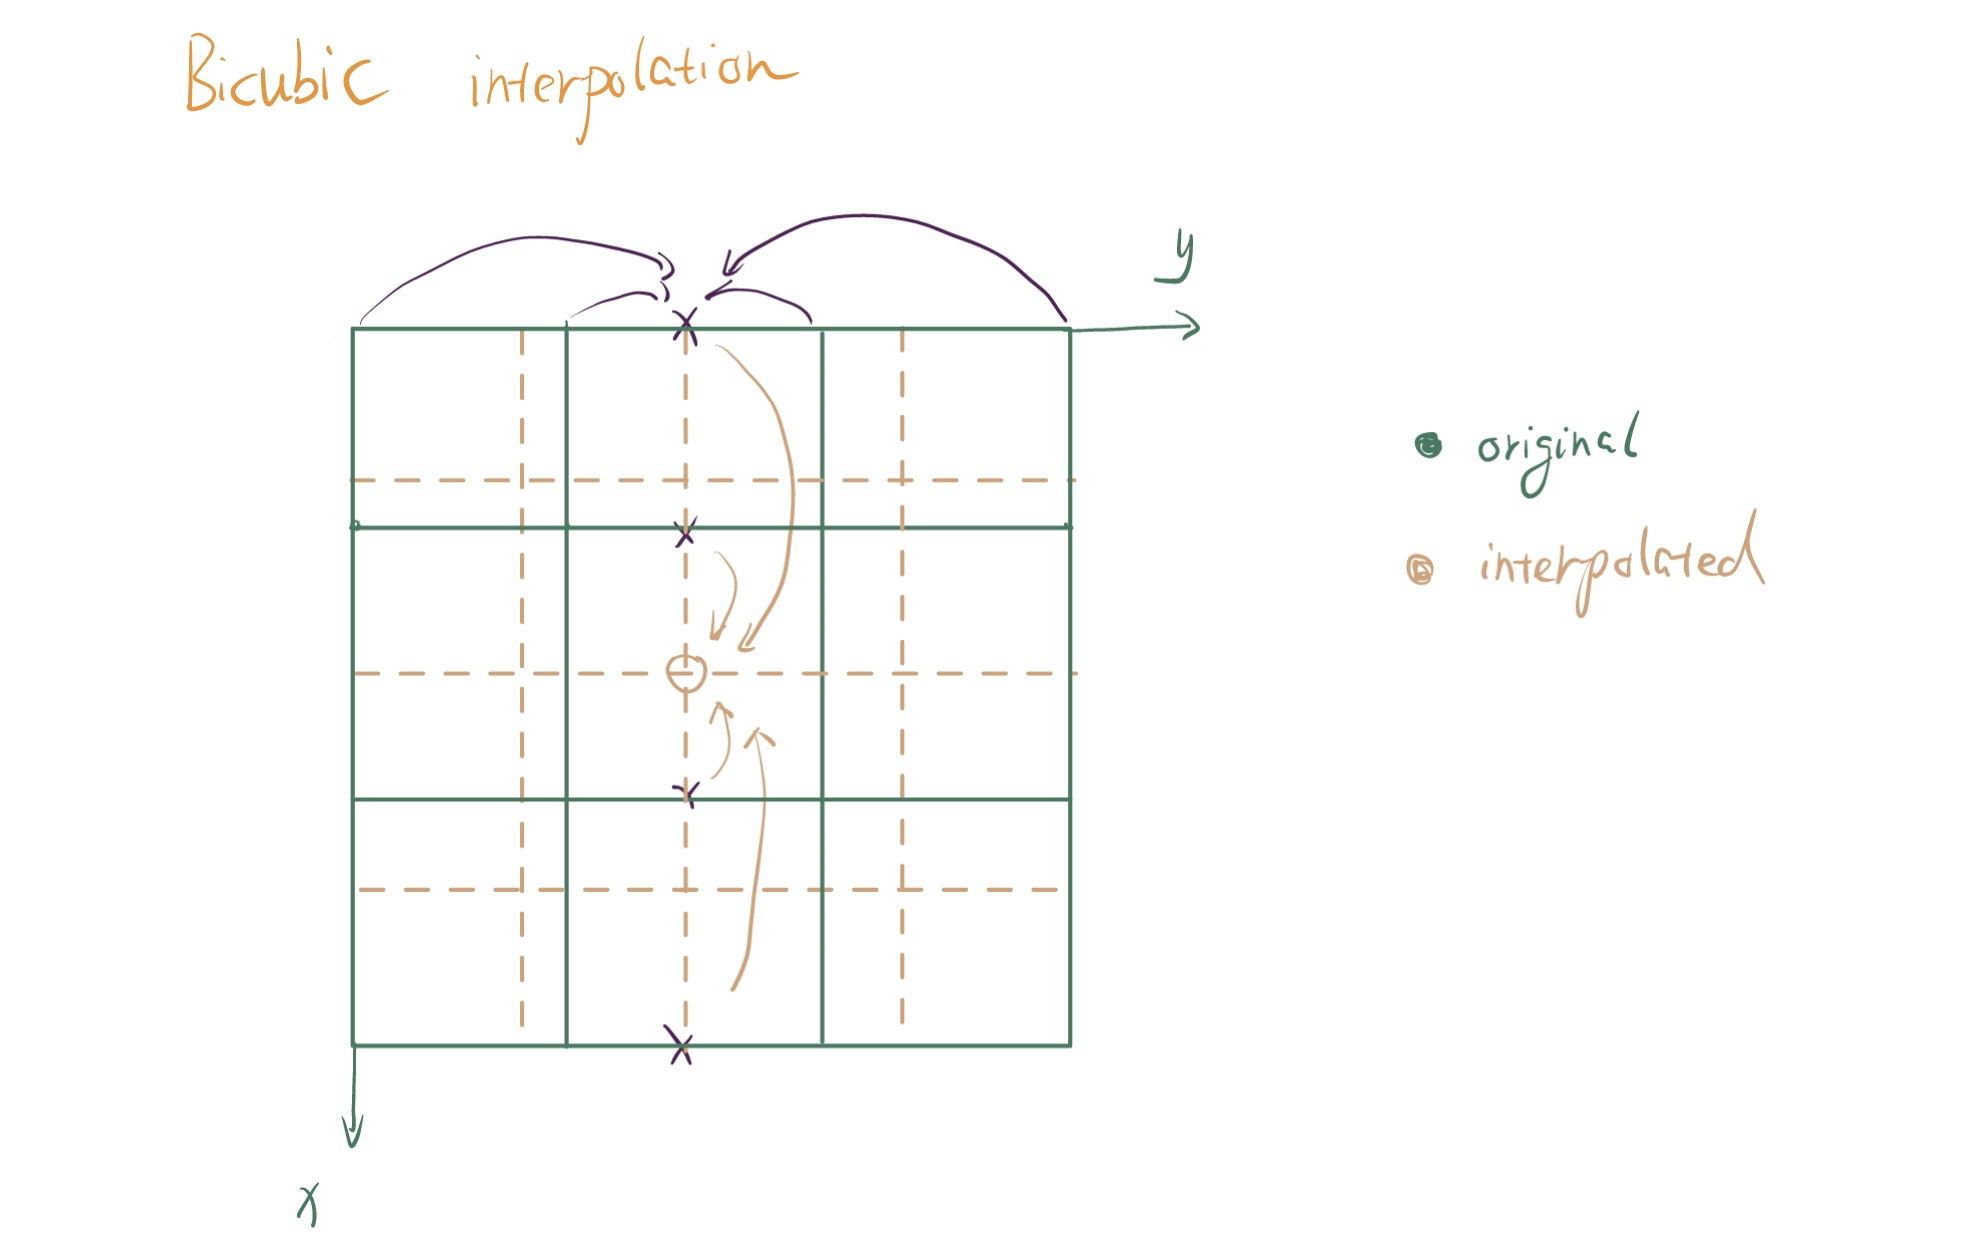
\includegraphics{D:/Tangent/SUSTech/大三下/课程资料/DIP/Lab/lab repo/Lab2/report/assets/bicubic_mapping.jpg}

As for the pixels close to the image edges, I flip the image along the
edges to fill up the ``outside pixels''. This can be easily done in
coding by flipping the index of those out of the bound.

\hypertarget{3-experiment}{%
\section{3 Experiment}\label{3-experiment}}

Note: The testing image for this section is Figure
\textbackslash ref\{\}.

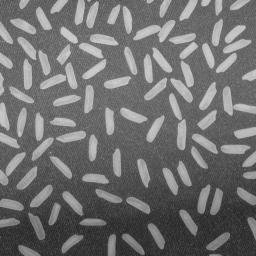
\includegraphics{D:/Tangent/SUSTech/大三下/课程资料/DIP/Lab/lab repo/Lab2/report/assets/rice_original.jpg}

\hypertarget{31-nearest-neighbor-interpolation}{%
\subsection{3.1 Nearest Neighbor
Interpolation}\label{31-nearest-neighbor-interpolation}}

The implementation of the nearest neighbor interpolation can be
expressed in the following pseudo code:

\begin{Shaded}
\begin{Highlighting}[]
\CommentTok{\# read the original image}
\NormalTok{img }\OperatorTok{=}\NormalTok{ read\_img(original\_img)}
\CommentTok{\# create a zero image array}
\NormalTok{out\_img.initialized(size }\OperatorTok{=}\NormalTok{ interpolated\_dim[}\DecValTok{0}\NormalTok{],interpolated\_dim[}\DecValTok{1}\NormalTok{])}
\CommentTok{\# traverse all the interpolated pixels}
\ControlFlowTok{for}\NormalTok{ x, y }\KeywordTok{in}\NormalTok{ out\_img:}
	\CommentTok{\# inverse mappping}
\NormalTok{	x1 }\OperatorTok{=}\NormalTok{ inverse\_mapping(x)}
\NormalTok{	y1 }\OperatorTok{=}\NormalTok{ inverse\_mapping(y)}

	\CommentTok{\#find the index of the nearest neighbor}
\NormalTok{	x2 }\OperatorTok{=} \BuiltInTok{round}\NormalTok{(x1)}
\NormalTok{	y2 }\OperatorTok{=} \BuiltInTok{round}\NormalTok{(y1)}
	
	\CommentTok{\#pixel assignment}
\NormalTok{	out\_img[x,y] }\OperatorTok{=}\NormalTok{ img[x2,y2]}
\ControlFlowTok{return}\NormalTok{ out\_img}
	
\end{Highlighting}
\end{Shaded}

\textbf{In particular, the inverse\_mapping() of three kinds of
interpolation is the same.} If written in \texttt{Python} language, it
should look like this:

\begin{Shaded}
\begin{Highlighting}[]
\NormalTok{x1 }\OperatorTok{=}\NormalTok{ x }\OperatorTok{*}\NormalTok{ (img.shape[}\DecValTok{0}\NormalTok{]}\OperatorTok{{-}}\DecValTok{1}\NormalTok{) }\OperatorTok{/}\NormalTok{ (dim[}\DecValTok{0}\NormalTok{] }\OperatorTok{{-}} \DecValTok{1}\NormalTok{)}
\NormalTok{y1 }\OperatorTok{=}\NormalTok{ y }\OperatorTok{*}\NormalTok{ (img.shape[}\DecValTok{1}\NormalTok{]}\OperatorTok{{-}}\DecValTok{1}\NormalTok{) }\OperatorTok{/}\NormalTok{ (dim[}\DecValTok{1}\NormalTok{] }\OperatorTok{{-}} \DecValTok{1}\NormalTok{)}
\end{Highlighting}
\end{Shaded}

Since the \texttt{round()} function in \texttt{Python} is already
searching for the nearest integer, we need not write another function to
do this.

The output image of the nearest neighbor interpolation looks something
like Figure \textbackslash ref\{\}.

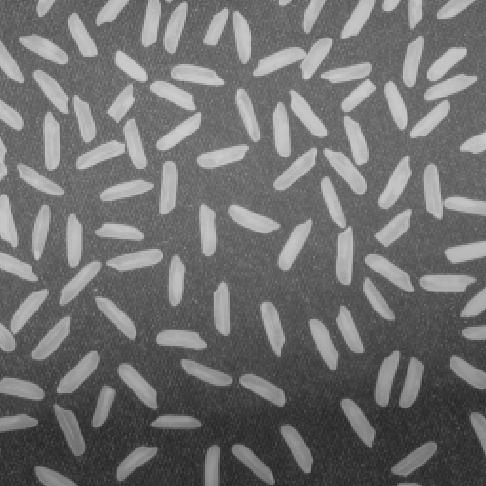
\includegraphics{D:/Tangent/SUSTech/大三下/课程资料/DIP/Lab/lab repo/Lab2/report/assets/rice_nearest.jpg}

\hypertarget{32-bilinear-interpolation}{%
\subsection{3.2 Bilinear
Interpolation}\label{32-bilinear-interpolation}}

In this part, since I have written two implementations for this method,
so there are two parts in this section.

\hypertarget{321-first-approach}{%
\subsubsection{3.2.1 First Approach}\label{321-first-approach}}

The first implementation of bilinear interpolation can be expressed in
the following pseudo-code, which performs two times linear
interpolation:

\begin{Shaded}
\begin{Highlighting}[]
\CommentTok{\# read the original image}
\NormalTok{img }\OperatorTok{=}\NormalTok{ read\_img(original\_img)}
\CommentTok{\# create a zero image array}
\NormalTok{out\_img.initialized(size }\OperatorTok{=}\NormalTok{ (interpolated\_dim[}\DecValTok{0}\NormalTok{],interpolated\_dim[}\DecValTok{1}\NormalTok{]))}
\CommentTok{\# create an intermediate image array}
\NormalTok{tmp.initialized(img.shape[}\DecValTok{0}\NormalTok{],interpolated\_dim[}\DecValTok{1}\NormalTok{])}

\CommentTok{\# first interpolate along the y{-}axis}
\ControlFlowTok{for}\NormalTok{ i,j }\KeywordTok{in}\NormalTok{ tmp:}
\NormalTok{    y }\OperatorTok{=}\NormalTok{ inverse\_mapping(j)}
\NormalTok{    y1 }\OperatorTok{=}\NormalTok{ floor(y1)}
\NormalTok{    tmp[i,j] }\OperatorTok{=}\NormalTok{ linear\_interp(img[i,y1],img[i,y1}\OperatorTok{+}\DecValTok{1}\NormalTok{],y)}

\CommentTok{\# then interpolate along the x{-}axis}
\ControlFlowTok{for}\NormalTok{ i, j }\KeywordTok{in}\NormalTok{ out\_img:}
\NormalTok{    x }\OperatorTok{=}\NormalTok{ inverse\_mapping(i)}
\NormalTok{    x1 }\OperatorTok{=}\NormalTok{ floor(x1)}
\NormalTok{    out\_img[i,j] }\OperatorTok{=}\NormalTok{ linear\_interp(img[x1,j],img[x1}\OperatorTok{+}\DecValTok{1}\NormalTok{,j],x)}

\NormalTok{returm out\_img}
\end{Highlighting}
\end{Shaded}

The \texttt{floor()} function returns the lower integer bound of the
input value.

And the \texttt{linear\_interp()} function written in \texttt{Python}
looks something like this:

\begin{Shaded}
\begin{Highlighting}[]
\ControlFlowTok{if}\NormalTok{ x1 }\OperatorTok{==}\NormalTok{ img.shape[}\DecValTok{0}\NormalTok{]}\OperatorTok{{-}}\DecValTok{1}\NormalTok{:}
\NormalTok{    x1 }\OperatorTok{{-}=} \DecValTok{1}
\NormalTok{out\_img[i,j] }\OperatorTok{=}\NormalTok{ tmp[x1,j] }\OperatorTok{+}\NormalTok{ (x}\OperatorTok{{-}}\NormalTok{x1)}\OperatorTok{*}\NormalTok{(tmp[x1}\OperatorTok{+}\DecValTok{1}\NormalTok{,j]}\OperatorTok{{-}}\NormalTok{tmp[x1,j])}
\end{Highlighting}
\end{Shaded}

Note that the first two lines of boundary detection are necessary.

The result of this implementation looks something like Figure
\textbackslash ref\{\}.

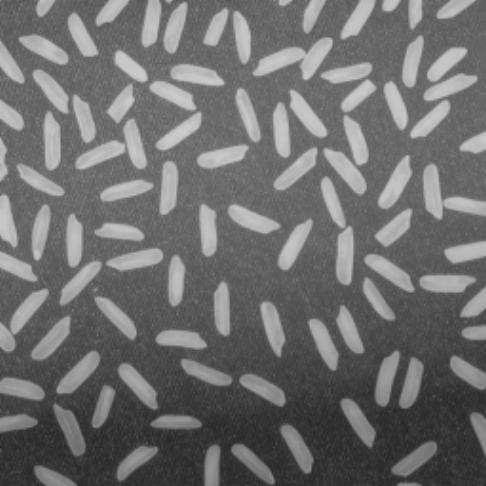
\includegraphics{D:/Tangent/SUSTech/大三下/课程资料/DIP/Lab/lab repo/Lab2/report/assets/rice_bilinear_original.jpg}

\hypertarget{322-second-approach}{%
\subsubsection{3.2.2 Second Approach}\label{322-second-approach}}

The second approach of bilinear interpolation directly computes the
output pixel value by using the four neighbors' values. The pseudo-code
of this implementation is as follows.

\begin{Shaded}
\begin{Highlighting}[]
\CommentTok{\# read the original image}
\NormalTok{img }\OperatorTok{=}\NormalTok{ read\_img(original\_img)}
\CommentTok{\# create a zero image array}
\NormalTok{out\_img.initialized(size }\OperatorTok{=}\NormalTok{ (interpolated\_dim[}\DecValTok{0}\NormalTok{],interpolated\_dim[}\DecValTok{1}\NormalTok{]))}

\ControlFlowTok{for}\NormalTok{ x,y }\KeywordTok{in}\NormalTok{ out\_img:}
\NormalTok{    x1, y1 }\OperatorTok{=}\NormalTok{ inverse\_mapping(x,y)}
\NormalTok{    m,n }\OperatorTok{=}\NormalTok{ calculate\_weight\_from\_index(x1,y1)}
\NormalTok{    out\_img[x,y] }\OperatorTok{=}\NormalTok{ weighted\_neighbor\_value(x1,y1,m,n)}
\ControlFlowTok{return}\NormalTok{ out\_img}
\end{Highlighting}
\end{Shaded}

In particular, the \texttt{calculate\_weight\_from\_index()} function
does the following jobs. The code is written in \texttt{Python}.

\begin{Shaded}
\begin{Highlighting}[]
\NormalTok{x1 }\OperatorTok{=}\NormalTok{ x }\OperatorTok{*}\NormalTok{ (img.shape[}\DecValTok{0}\NormalTok{]}\OperatorTok{{-}}\DecValTok{1}\NormalTok{) }\OperatorTok{/}\NormalTok{ (dim[}\DecValTok{0}\NormalTok{] }\OperatorTok{{-}} \DecValTok{1}\NormalTok{)}
\NormalTok{x2 }\OperatorTok{=}\NormalTok{ math.floor(x1)}
\NormalTok{m }\OperatorTok{=}\NormalTok{ x1 }\OperatorTok{{-}}\NormalTok{ x2}
\NormalTok{y1 }\OperatorTok{=}\NormalTok{ y }\OperatorTok{*}\NormalTok{ (img.shape[}\DecValTok{1}\NormalTok{]}\OperatorTok{{-}}\DecValTok{1}\NormalTok{) }\OperatorTok{/}\NormalTok{ (dim[}\DecValTok{1}\NormalTok{] }\OperatorTok{{-}} \DecValTok{1}\NormalTok{)}
\NormalTok{y2 }\OperatorTok{=}\NormalTok{ math.floor(y1)}
\NormalTok{n }\OperatorTok{=}\NormalTok{ y1 }\OperatorTok{{-}}\NormalTok{ y2}
\end{Highlighting}
\end{Shaded}

And the \texttt{weighted\_neighbor\_value()} function calculates the
final pixel's value:

\begin{Shaded}
\begin{Highlighting}[]
\NormalTok{out\_img[x, y] }\OperatorTok{=}\NormalTok{ (}\DecValTok{1}\OperatorTok{{-}}\NormalTok{n) }\OperatorTok{*}\NormalTok{ (m }\OperatorTok{*}\NormalTok{ img[x2}\OperatorTok{+}\DecValTok{1}\NormalTok{,y2] }\OperatorTok{+}\NormalTok{ (}\DecValTok{1}\OperatorTok{{-}}\NormalTok{m) }\OperatorTok{*}\NormalTok{ img[x2,y2])}\OperatorTok{+}\NormalTok{ n }\OperatorTok{*}\NormalTok{ (m }\OperatorTok{*}\NormalTok{ img[x2}\OperatorTok{+}\DecValTok{1}\NormalTok{,y2}\OperatorTok{+}\DecValTok{1}\NormalTok{] }\OperatorTok{+}\NormalTok{ (}\DecValTok{1}\OperatorTok{{-}}\NormalTok{m)}\OperatorTok{*}\NormalTok{img[x2,y2}\OperatorTok{+}\DecValTok{1}\NormalTok{])}
\end{Highlighting}
\end{Shaded}

The resulting interpolated image of this approach looks something like
Figure \textbackslash ref\{\}, which is the same as Figure
\textbackslash ref\{\}.

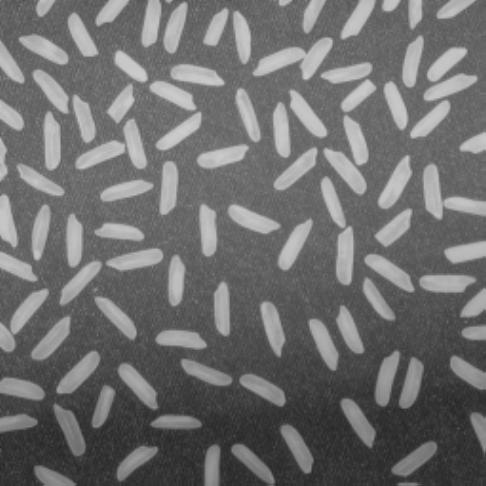
\includegraphics{D:/Tangent/SUSTech/大三下/课程资料/DIP/Lab/lab repo/Lab2/report/assets/rice_bilinear.jpg}

\hypertarget{33-bicubic-interpolation}{%
\subsection{3.3 Bicubic Interpolation}\label{33-bicubic-interpolation}}

The pseudo-code for bicubic interpolation is as follows:

\begin{Shaded}
\begin{Highlighting}[]
\CommentTok{\# read the original image}
\NormalTok{img }\OperatorTok{=}\NormalTok{ read\_img(original\_img)}
\CommentTok{\# create a zero image array}
\NormalTok{out\_img.initialized(size }\OperatorTok{=}\NormalTok{ (interpolated\_dim[}\DecValTok{0}\NormalTok{],interpolated\_dim[}\DecValTok{1}\NormalTok{]))}
\CommentTok{\# create an intermediate image array}
\NormalTok{tmp.initialized(interpolated\_dim[}\DecValTok{0}\NormalTok{],img.shape[}\DecValTok{1}\NormalTok{])}

\CommentTok{\# first interpolate along x{-}axis}
\ControlFlowTok{for}\NormalTok{ x, y }\KeywordTok{in}\NormalTok{ tmp:}
\NormalTok{    x1 }\OperatorTok{=}\NormalTok{ inverse\_mapping(x)}
\NormalTok{    sample\_x }\OperatorTok{=}\NormalTok{ [floor(x1)}\OperatorTok{{-}}\DecValTok{1}\NormalTok{,floor(x1),floor(x1)}\OperatorTok{+}\DecValTok{1}\NormalTok{,floor(x1)}\OperatorTok{+}\DecValTok{2}\NormalTok{]}
\NormalTok{    sample\_y }\OperatorTok{=}\NormalTok{ find\_pixel\_value\_of\_sample\_x(flip\_if\_needed(sample\_x))}
\NormalTok{    cubic\_func }\OperatorTok{=}\NormalTok{ fit\_cubic\_function(sample\_x,sample\_y)}
\NormalTok{    tmp[x, y] }\OperatorTok{=}\NormalTok{ cubic\_func(x1)}

\CommentTok{\# then interpolate along y{-}axis}
\ControlFlowTok{for}\NormalTok{ x, y }\KeywordTok{in}\NormalTok{ out\_img:}
\NormalTok{    y1 }\OperatorTok{=}\NormalTok{ inverse\_mapping(y)}
\NormalTok{    sample\_y }\OperatorTok{=}\NormalTok{ [floor(y1)}\OperatorTok{{-}}\DecValTok{1}\NormalTok{,floor(y1),floor(y1)}\OperatorTok{+}\DecValTok{1}\NormalTok{,floor(y1)}\OperatorTok{+}\DecValTok{2}\NormalTok{]}
\NormalTok{    sample\_x }\OperatorTok{=}\NormalTok{ find\_pixel\_value\_of\_sample\_y(flip\_if\_needed(sample\_x))}
\NormalTok{    cubic\_func }\OperatorTok{=}\NormalTok{ fit\_cubic\_function(sample\_x,sample\_y)}
\NormalTok{    out\_img[x, y] }\OperatorTok{=}\NormalTok{ cubic\_func(y1)}

\ControlFlowTok{return}\NormalTok{ out\_img}
\end{Highlighting}
\end{Shaded}

The \texttt{flip\_if\_needed()} function can handle the case that the
requested index of the original pixel is out of bounds. It looks
something like this if written in \texttt{Python} code:

\begin{Shaded}
\begin{Highlighting}[]
\CommentTok{\# find the nearest orginial pixel index}
\NormalTok{m }\OperatorTok{=}\NormalTok{ np.array([np.floor(x1)}\OperatorTok{{-}}\DecValTok{1}\NormalTok{, np.floor(x1), np.floor(x1)}\OperatorTok{+}\DecValTok{1}\NormalTok{, np.floor(x1)}\OperatorTok{+}\DecValTok{2}\NormalTok{])}
\NormalTok{m\_tmp }\OperatorTok{=}\NormalTok{ m.copy()}
\NormalTok{m\_tmp[m\_tmp }\OperatorTok{\textless{}} \DecValTok{0}\NormalTok{] }\OperatorTok{=}\NormalTok{ np.}\BuiltInTok{abs}\NormalTok{(m\_tmp[m\_tmp }\OperatorTok{\textless{}} \DecValTok{0}\NormalTok{])}
\NormalTok{m\_tmp[m\_tmp }\OperatorTok{\textgreater{}=}\NormalTok{ img.shape[}\DecValTok{0}\NormalTok{]] }\OperatorTok{=} \DecValTok{2}\OperatorTok{*}\NormalTok{img.shape[}\DecValTok{0}\NormalTok{] }\OperatorTok{{-}}\NormalTok{ m\_tmp[m\_tmp }\OperatorTok{\textgreater{}=}\NormalTok{ img.shape[}\DecValTok{0}\NormalTok{]] }\OperatorTok{{-}} \DecValTok{1}
\NormalTok{m\_tmp }\OperatorTok{=}\NormalTok{ m\_tmp.astype(}\BuiltInTok{int}\NormalTok{)}
\end{Highlighting}
\end{Shaded}

And I fit a cubic function using the \texttt{polyfit} and
\texttt{poly1d} function in \texttt{numpy}, which in code are something
like this:

\begin{Shaded}
\begin{Highlighting}[]
\NormalTok{coefficients }\OperatorTok{=}\NormalTok{ np.polyfit(m, n, }\DecValTok{3}\NormalTok{)}
\NormalTok{poly }\OperatorTok{=}\NormalTok{ np.poly1d(coefficients)}
\NormalTok{tmp[x, y] }\OperatorTok{=}\NormalTok{ poly(x1)}
\end{Highlighting}
\end{Shaded}

Here, \texttt{m} and \texttt{n} are the \texttt{sample\_x} and
\texttt{sample\_y} in the pseudo-code.

The resulting image of bicubic interpolation is Figure
\textbackslash ref\{\}.

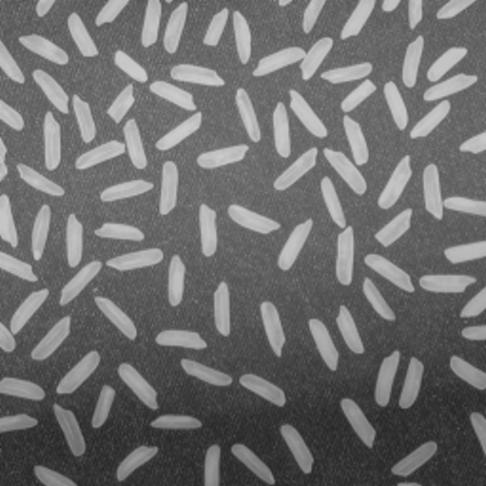
\includegraphics{D:/Tangent/SUSTech/大三下/课程资料/DIP/Lab/lab repo/Lab2/report/assets/rice_bicubic.jpg}

\hypertarget{4-result-analysis}{%
\section{4 Result Analysis}\label{4-result-analysis}}

From the above Figure \textbackslash ref\{\} to Figure
\textbackslash ref\{\}, we can intuitively understand these three
interpolation methods.

For nearest neighbor interpolation, the edgy effect is because nearby
pixels in the interpolated image can be assigned to different neighbors
in the original image, and this causes the neighbor of the interpolated
image to have mutated values.

For bilinear interpolation, since it considers the linear change in both
directions, the interpolated image should have a smooth transition from
pixel to pixel. However, this can also make the output image look
blurry.

For bicubic interpolation, it considers more nearby pixels during the
interpolation process to capture the inner nature of change of the
original image, giving the interpolated image a sharper outline.

To better compare the efficiency of all of the above interpolations as
well as a \texttt{scipy} implemented bicubic interpolation, I do a
timing benchmark, the result is as follows:

\begin{Shaded}
\begin{Highlighting}[]
\NormalTok{Nearest: }\FloatTok{0.17167043685913086}\NormalTok{ seconds.}
\NormalTok{Bilinear type1: }\FloatTok{0.12122154235839844}\NormalTok{ seconds.}
\NormalTok{Bilinear type2: }\FloatTok{1.1743693351745605}\NormalTok{ seconds.}
\NormalTok{Bicubic: }\FloatTok{16.160951852798462}\NormalTok{ seconds.}
\NormalTok{Bicubic Scipy: }\FloatTok{0.00809168815612793}\NormalTok{ seconds.}
\end{Highlighting}
\end{Shaded}

The bicubic interpolation I wrote is the slowest, which is in accord
with my expectation because it involves so many regressions. And since
\texttt{scipy} is a library highly optimized for science computation, it
should have the best record.

However, I expected the bilinear interpolation in section 3.2.1 to be
less efficient than the one in section 3.2.2, because the first approach
involves 2 \texttt{for} loops while the second approach only involves 1
\texttt{for} loop, while the timing benchmark is against my intuition.
So I tried to do some simple ablation study.

I found that if I comment out all the pixel assignment statements,
approach 2 runs faster than approach.

\begin{Shaded}
\begin{Highlighting}[]
\NormalTok{Bilinear type1: }\FloatTok{0.11931777000427246}\NormalTok{ seconds.}
\NormalTok{Bilinear type2: }\FloatTok{0.08695650100708008}\NormalTok{ seconds.}
\end{Highlighting}
\end{Shaded}

Hence, the bottleneck of approach 2 is this statement:

\begin{Shaded}
\begin{Highlighting}[]
\NormalTok{out\_img[x, y] }\OperatorTok{=}\NormalTok{ (}\DecValTok{1}\OperatorTok{{-}}\NormalTok{n) }\OperatorTok{*}\NormalTok{ (m }\OperatorTok{*}\NormalTok{ img[x2}\OperatorTok{+}\DecValTok{1}\NormalTok{,y2] }\OperatorTok{+}\NormalTok{ (}\DecValTok{1}\OperatorTok{{-}}\NormalTok{m) }\OperatorTok{*}\NormalTok{ img[x2,y2])}\OperatorTok{+}\NormalTok{ n }\OperatorTok{*}\NormalTok{ (m }\OperatorTok{*}\NormalTok{ img[x2}\OperatorTok{+}\DecValTok{1}\NormalTok{,y2}\OperatorTok{+}\DecValTok{1}\NormalTok{] }\OperatorTok{+}\NormalTok{ (}\DecValTok{1}\OperatorTok{{-}}\NormalTok{m)}\OperatorTok{*}\NormalTok{img[x2,y2}\OperatorTok{+}\DecValTok{1}\NormalTok{])}
\end{Highlighting}
\end{Shaded}

I guess that this statement runs so slowly due to the nature of memory,
which means the process of accessing those pixel values in array
\texttt{img} is not continuous.

\hypertarget{5-conclusion}{%
\section{5 Conclusion}\label{5-conclusion}}

In this lab, we explore three types of interpolation methods: nearest
neighbor interpolation, bilinear interpolation, and bicubic
interpolation. We first analyze the mathematic derivation of these
interpolation methods. Then, we analyze the interpolation effects by
looking into the images these interpolation methods produced and finding
the root of these differences. Finally, we do a timing benchmark of this
method and discover the efficiency difference between these methods. In
particular, we try two implementations of bilinear interpolation,
distinguishing their efficiency difference.

\end{document}
